\chapter{EvoOracle: LLMs for Oracles}
\label{cha:evoOracles}
\vspace{0.4 cm}

In this chapter, we introduce EvoOracle, our innovative tool designed for efficient oracle generation using Large Language Models (LLMs). Figure 4.1 provides an insightful overview of EvoOracle's key components and workflow. To initiate the process, we acquire a dataset of Java open-source projects sourced from GitHub. Employing automated test case generation tools such as EvoSuite and Randoop, we systematically create Automated JUnit Test Cases for each project, laying the foundation for EvoOracle's subsequent operations. The tool begins by extracting metadata linked to the identified classes and methods within each project. Subsequently, it mines test cases and establishes mappings with corresponding focal methods extracted from the earlier project analysis. The SUT (System Under Test) Processor component plays a pivotal role in this phase, removing assertions from the test cases and substituting them with placeholders. Following this, the Prompt Processor component takes these test cases, now equipped with placeholders and focal methods, and formulates context for LLM prompting. The LLM Query Processor component utilizes this context to prompt the LLMs, passing the generated responses to the LLM Response Handler component. This handler, in turn, readies the test cases for execution. Finally, the Test Executor compiles and executes the newly generated tests, completing the comprehensive cycle of EvoOracle's oracle generation process.

\begin{figure}[H]
\centering
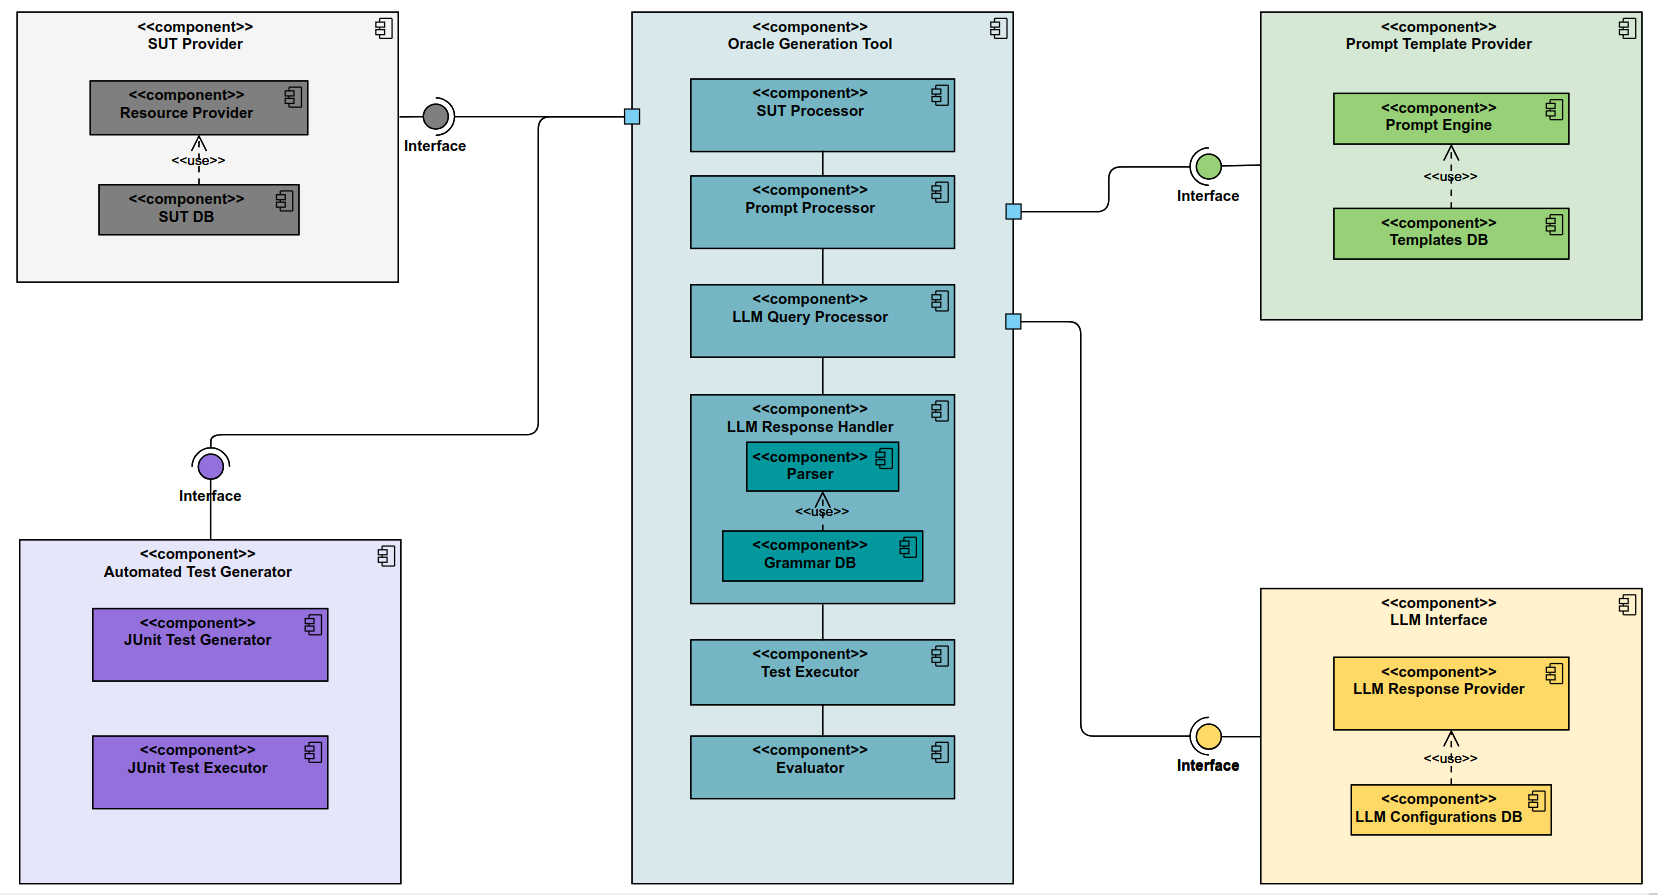
\includegraphics[width=1\textwidth]{images/UML_Component_Diagram_EvoOracle_v2.png}
\caption{Components of our proposed tool: EvoOracle}
\label{fig:component_diagram}
\end{figure}

In the following sub-chapters, we will delve into the intricacies of each step, providing detailed descriptions and insights into the nuances of EvoOracle's comprehensive process.

\section{Data Collection}
\label{sec:data_collection}
\vspace{0.2 cm}
Within this sub-chapter, we will elaborate on our methodology for assembling a collection of Java projects. We outline the procedures involved in generating test cases using automated tools such as EvoSuite and Randoop\cite{noauthor_randoop_nodate}, shedding light on the meticulous steps taken to ensure comprehensive test coverage. Additionally, we will discuss the meticulous process of preparing corresponding focal methods, elucidating how we identify and associate the specific methods targeted by each test case. This step is crucial in establishing a robust foundation for subsequent analyses and evaluations within the realm of software testing and development.

\vspace{0.1 cm}
\subsection{Java Projects Selection}
\label{sec:projects_selection}
\vspace{0.1 cm}

We carefully selected four projects, as outlined in Table \ref{tab:collected_java_projects}, from the pool of publicly available GitHub Java repositories that declare an open-source license. To ensure relevance and avoid potential data leakage, we specifically focused on projects updated within the last three years. Our selection criteria also considered popularity, with priority given to projects boasting the highest number of stars or forks. Emphasizing diversity, we aimed to cover a spectrum of project types. From these chosen projects, encompassing a total of 388 classes, we further refined our sample by randomly selecting nine classes, totaling 87 methods. This thoughtful selection process ensures that our tool encounters a diverse range of scenarios and project structures, contributing to a more comprehensive evaluation. Further details about these chosen classes can be found in Table \ref{tab:selected_java_projects}.

\begin{table}
    \centering
    \begin{tabular}{l | l | r}
        \textbf{Project Name} & \textbf{Classes} & \textbf{Reference} \\
        \hline
        frontend-maven-plugin & 43 & \cite{sletteberg_frontend-maven-plugin_2023} \\
        javacv & 117 & \cite{noauthor_bytedecojavacv_nodate} \\
        webdrivermanager & 44 & \cite{noauthor_bonigarciawebdrivermanager_nodate} \\
        zerocode & 184 & \cite{noauthor_authorjappszerocode_nodate} \\
    \end{tabular}
\caption{Details of the collected Java projects.}
\label{tab:collected_java_projects}
\end{table}

\begin{table}
    \centering    
    \begin{tabular}{l | l | r}
        \textbf{Class Name} & \textbf{Project Name} & \textbf{Methods} \\
        \hline
        BaseSettings & javacv & 6 \\
        Parallel & javacv & 6 \\
        SeekableByteArrayOutputStream & javacv & 3 \\
        NPMInstaller & frontend-maven-plugin & 15 \\
        NodeInstaller & frontend-maven-plugin & 18 \\
        PnpmInstaller & frontend-maven-plugin & 14 \\
        CacheHandler & webdrivermanager & 4 \\
        PropertiesProviderUtils & zerocode & 4 \\
        ZerocodeCorrelationshipLogger & zerocode & 17 \\
    \end{tabular}
\caption{Summary of selected Java projects.}
\label{tab:selected_java_projects}
\end{table}

\vspace{0.1 cm}
\subsection{Test Case Generation with EvoSuite}
\label{sec:test_case_generation}
\vspace{0.1 cm}

Our tool is designed to enhance existing test cases by focusing on improving assertions. To achieve this, we require one or more test suites, and for our research, we've opted to use EvoSuite. EvoSuite\cite{noauthor_evosuite_nodate} is a sophisticated tool specifically tailored for automatically generating test cases with assertions for Java code. It employs a unique hybrid approach that not only generates but also optimizes entire test suites to fulfill specific coverage criteria. These criteria guide the tool in producing comprehensive test suites that effectively cover the targeted code. EvoSuite doesn't stop at merely generating tests; it goes a step further by suggesting potential oracles for these test cases. Oracles, in this context, are sets of assertions strategically added to succinctly summarize the current behavior of the code. These assertions serve a crucial role—enabling developers to identify deviations from expected behavior and capturing the existing behavior to safeguard against potential defects in the future.

For our study, we utilized EvoSuite to generate automated test cases for each of the selected classes. We adhered to the default configurations of EvoSuite, setting the search budget to 15 and opting not to minimize. We generated 9 Test Suites with a total of 138 test cases. The generated test suites for each class are outlined in Table \ref{tab:evosuite_testclasses}.

\begin{table}
    \centering    
    \begin{tabular}{l | l | r}
        \textbf{Test Suite} & \textbf{Class Name} & \textbf{Test Cases} \\
        \hline
        BaseSettings\_ESTest & BaseSettings & 14 \\
        Parallel\_ESTest & Parallel & 6 \\
        SeekableByteArrayOutputStream\_ESTest & SeekableByteArrayOutputStream & 13 \\
        NPMInstaller\_ESTest & NPMInstaller & 18 \\
        NodeInstaller\_ESTest & NodeInstaller & 18 \\
        PnpmInstaller\_ESTest & PnpmInstaller & 21 \\
        CacheHandler\_ESTest & CacheHandler & 13 \\
        PropertiesProviderUtils\_ESTest & PropertiesProviderUtils & 14 \\
        ZerocodeCorrelationshipLogger\_ESTest & ZerocodeCorrelationshipLogger & 21 \\
    \end{tabular}
\caption{Summary of EvoSuite generated test classes.}
\label{tab:evosuite_testclasses}
\end{table}

\vspace{0.1 cm}
\subsection{Metadata Extraction}
\label{sec:data_extraction}
\vspace{0.1 cm}

This step involves parsing each project to extract essential information about classes and methods, along with their associated metadata. Once this information is obtained, our focus shifts to identifying test classes and establishing their connections with corresponding focal classes. This pivotal step ensures that we precisely match each test class with its relevant counterpart. Following the identification of test classes and their associations, we move on to a crucial mapping process. For every test case within a test class, we meticulously map it to the corresponding focal method. This meticulous mapping results in a comprehensive set of mapped test cases, forming the foundation for subsequent stages in our methodology.

\begin{itemize}
  \item \textbf{Parsing:} In the parsing phase, we thoroughly analyze each project using the tree-sitter parser\cite{noauthor_tree-sitterintroduction_nodate}. This process involves extracting valuable metadata linked to the identified classes and methods within the project. The collected information encompasses crucial details like class names, signatures, super class, bodies, annotations, interfaces, package, imports, fields, arguments list, constructors, dependencies and variables, method names, return types, any developer written comments. This parsed code serves a dual purpose: firstly, to pinpoint test cases and their corresponding focal methods, and secondly, to enhance the focal methods by incorporating focal context information.
                                
  \item \textbf{Identify Test Classes:} In this stage, our goal is to locate all the test classes within the project. Test classes are those classes housing at least one method annotated with the \textit{\textbf{@Test}} annotation. This specific annotation serves as an indicator to JUnit, signaling that the attached method is eligible to be executed as a test case. By identifying and marking classes in this manner, we establish a clear distinction between regular classes and those instrumental to the testing process. This categorization allows a systematic approach to handling test-related components.

  \item \textbf{Identify Focal Classes:} Identifying Focal Classes involves determining the class under test for each test class. We employ a two-step approach using the following heuristics:
        \begin{enumerate}
            \item \textbf{Extracting Class Instances:} The initial heuristic involves analyzing each test method to identify all the classes instantiated or any objects created during the testing process.
            \item \textbf{Matching Class Names:} Subsequently, we employ name matching as the second heuristic. Test classes typically follow a naming convention that includes the name of the focal class, often with a \textit{"Test"} prefix or suffix. For instance, a test class associated with the \textit{"BaseSettings.java"} class might be named \textit{"BaseSettingsTest.java"} or, in the case of Evosuite, \textit{"BaseSettings\_ESTest.java."} To identify the focal class, we perform name matching by comparing the name of the test class (minus the optional \textit{"\_ESTest"} suffix) with potential focal classes. This step ensures a robust association between test classes and their corresponding focal classes.
        \end{enumerate}

  \item \textbf{Identify Focal Method:} Determining the focal method for each test case involves employing specific heuristics. 
  \begin{enumerate}
      \item \textbf{Matching Method Names:} This heuristic leverages the common practice of naming test cases similarly to their corresponding focal methods. This involves matching test case names with focal methods, considering potential prefixes or suffixes like "Test."
      \item \textbf{Analyzing Method Invocations:} Additionally, this heuristic is applied if the initial method doesn't identify a focal method. We try to match the method invocations within the test case and the methods defined in the focal class. If a match is found, it is selected as the focal method. This approach is grounded in the confidence gained from prior matching of the test class to the focal class, making it likely that the test case is specifically targeting that single method.
  \end{enumerate}

  Following these heuristics, we obtain a set of test cases paired with their corresponding focal class and focal methods. Test cases where we couldn't identify the focal method using our heuristics are excluded from further consideration.
  
\end{itemize}

\section{Preprocessing}
\label{sec:preprocessing}
\vspace{0.2 cm}

In this section, ...

\vspace{0.1 cm}
\subsection{Removal of Assertions from Test Cases}
\label{sec:assertion_removal}
\vspace{0.1 cm}

In this subsection, an overview of ...

\vspace{0.1 cm}
\subsection{Placeholder Insertion}
\label{sec:placeholder_insertion}
\vspace{0.1 cm}

In this subsection, ...

\section{Large Language Model Integration}
\label{sec:llm_integration}
\vspace{0.2 cm}

In this section, ...

\vspace{0.1 cm}
\subsection{LLM Selection and Configuration}
\label{sec:llm_configurations}
\vspace{0.1 cm}

In this subsection, an overview of ...

\vspace{0.1 cm}
\subsection{Prompt Preparation}
\label{sec:prompt_preparation}
\vspace{0.1 cm}

In this subsection, ...

\vspace{0.1 cm}
\subsection{Generating Assertions}
\label{sec:generating_assertions}
\vspace{0.1 cm}

In this subsection, ...

\vspace{0.1 cm}
\subsection{Evaluating Response Quality}
\label{sec:evaluating_response}
\vspace{0.1 cm}

In this subsection, ...

\section{Test Case Preparation}
\label{sec:test_case_preparation}
\vspace{0.2 cm}

In this section, ...

\vspace{0.1 cm}
\subsection{Assertion Integration}
\label{sec:assertion_integration}
\vspace{0.1 cm}

In this subsection, ...

\vspace{0.1 cm}
\subsection{Test Case Compilation}
\label{sec:test_compilation}
\vspace{0.1 cm}

In this subsection, an overview of ...